\chapter{Transforming Raw Data to structured format}
\section*{Extract, Load, Transform}
Raw data from the experiment is stored in \gls{HDF5} files. This includes many \gls{beamline} diagnostic information such as \gls{BAM}, \gls{GMD}, the delay stage readings, the monochromator energy, sample specific information such as extractor voltage, and the electron counting in the 3 detector dimensions corresponding to the \gls{DLD} spatial X and Y axes and the temporal time axis. This information is resolved at each bunch of electrons coming from the accelerator called a \gls{train}, which are further microbunched into \glsplural{pulse}.

The \gls{OpenCOMPES} was established to develop tools and infrastructure to make analysis easier. To this end, a modular Python library called \texttt{\gls{SED}} was created that provides the entire pipeline from easy data ingestion to common calibration and corrections, multidimensional binning to create images, and saving the images to standard formats, with proper care of data provenance.

The data pipeline follows an ELT (Extract, Load, Transform) process, wherein raw data is extracted from \gls{HDF5} files, transformed into a structured format suitable for analysis, and subsequently stored in intermediate buffer files for further downstream processes such as analysis and visualization.

The following sections provide a detailed exposition of each stage of this ELT process. The first stage, extraction, begins with the loading of raw data from the \gls{HDF5} files. These files encapsulate experimental results across multiple channels, including electron-resolved and time-resolved data. The hierarchical structure of the \gls{HDF5} files allows the organization of data into groups, where each group contains an index and its corresponding dataset, collectively referred to as a “channel” The paths to these \gls{HDF5} files, along with relevant configuration parameters, are provided to the pipeline to dictate the steps of the subsequent transformation process.

\section*{Pipeline Overview}
To optimize performance and facilitate data management, the pipeline generates buffer files for each type of data (electron and time-resolved). This task is handled by the \texttt{BufferFilePaths} class, which initializes file paths and manages the creation of buffer files in the efficient \texttt{Parquet} format. By checking the presence of pre-existing buffer files, the class determines whether to reuse these files or regenerate them, based on the \texttt{force\_recreate} flag.

Each \gls{HDF5} file results in the generation of two primary buffer files: one containing electron-resolved data and another containing pulse/train-resolved data. These files are essential for organizing the data at the pulse level and maintaining resolution at the electron level. The data for each train contains roughly 500 pulses, and although some data is resolved at the pulse level, each index often holds an array, necessitating the use of the \texttt{pandas} MultiIndex functionality to maintain the data’s hierarchical structure. Detector measurements, which are electron-resolved along the X, Y, and temporal axes, are typically represented as three-dimensional arrays and add further complexity to the indexing process.

A critical transformation step involves correcting for offsets in pulse IDs to ensure accurate synchronization of data across different channels. Any data associated with pulse IDs below zero is removed, as it is considered invalid. Similarly, \texttt{NaN} pulses are dropped to avoid introducing inconsistencies in downstream analyses. While it is possible that pulses exceeding 500 may also be invalid, these are not filtered during this stage, as that determination is deferred to the final analysis. Due to machine fluctuations, pulses may become unsorted, and hence the pulses are sorted within each train to maintain temporal order.

Once this cleaning process is completed, electron-resolved channels are combined using an outer join with pulse and train-resolved channels, forming a comprehensive dataframe that contains all relevant information for further analysis. This merged dataset is separated into two primary dataframes: the electron-resolved dataframe and the pulse-resolved dataframe.

The electron dataframe contains only rows where electron events have been detected, with any missing data in non-electron channels forward-filled to ensure completeness. This dataframe serves as the main source of electron-specific data for further analyses. However, given that not all pulses or trains may produce electron events, a separate pulse-resolved dataframe is generated to capture all available train and pulse data, independent of electron detections. This pulse-resolved dataframe is essential for normalization steps involving time-resolved channels, such as those related to the delay axis.

The pipeline also includes validation steps for auxiliary channels, particularly those containing multi-dimensional data (e.g., 4D arrays), ensuring that all required channels exist within the files before proceeding with further transformations.

After this initial transformation and extraction, the buffer files are saved in \texttt{Parquet} format, chosen for its efficiency in storage and speed of access during future computations. The final stage involves the loading of all these buffer files into a unified dataframe using \texttt{Dask}, a distributed computing library that enables scalable processing of large datasets. At this stage, forward-filling is again applied to non-electron channels, ensuring that missing values between files are handled consistently. However, care must be taken when forward-filling across different runs, as this could introduce inter-run inconsistencies.

Finally, the schema of the buffer files is cross-validated against the predefined list of channels to ensure consistency and completeness prior to loading the data into \texttt{Dask}.


% At \gls{FLASH}, the data \gls{trARPES}
% Each file:
% Train indexed data is stored in HDF5 files. Index and data itself are stored in two separate HDF groups.
% Each pair is called channel. Load relevant channels. ~500 pulses each train. Some data is stored as pulse resolved but each index has an array
% so pandas Multiindex is used to create heirarchy. Detector measurements such as the X Y and TOF are electron resolved. So they are a 3d array and that can have another level of index then. There is an offset in pulseId so that no measurements are missed. This offset is first corrected. All data is below pulse 0 is removed as it is invalid. All nan pulses are also dropped. We do not filter above 500 even though those might also be invalid but leave that to end analysis. Pulses are sorted as due to machine, they might have bits moved around.
% Electron resolved channels are then combined together as they have the same index. THese channels are outer joined with the pulse and train resolved data (the slower frequency channels) to create a dataframe. 

% Two dataframes from this are created, an electron dataframe and a pulse resolved dataframe.
% All non-electron channels are forward filled. After this, all rows without an electron event are dropped. This is the electorn dataframe.

% It's possible that not all pulses/trains produce an electron and hence the pulse and train resolved channels with that information would not be available in the electron dataframe. So another dataframe that is containing all trains and pulses but is not electron reolsved is created called the timed dataframe. This is used to normalize by the delay axis for example
% Aux channel treatment (4d array)

% Channels groups are first validated if they exist in the file.


% This reduction process is done for all files and they are saved as parquet (buffer) since it is storage efficient and fast to read.

% We load all these files as one dataframe dask, a distributed computing python library. These files are again forward filled for each dataframe (only non-electron channels) to fill the interfile values. Probably wrong to fill different runs.

% The schema of the buffer files is checked against the list of channels before loading the data to dask.

\begin{figure}
    \label{fig:elt}
    \centering
    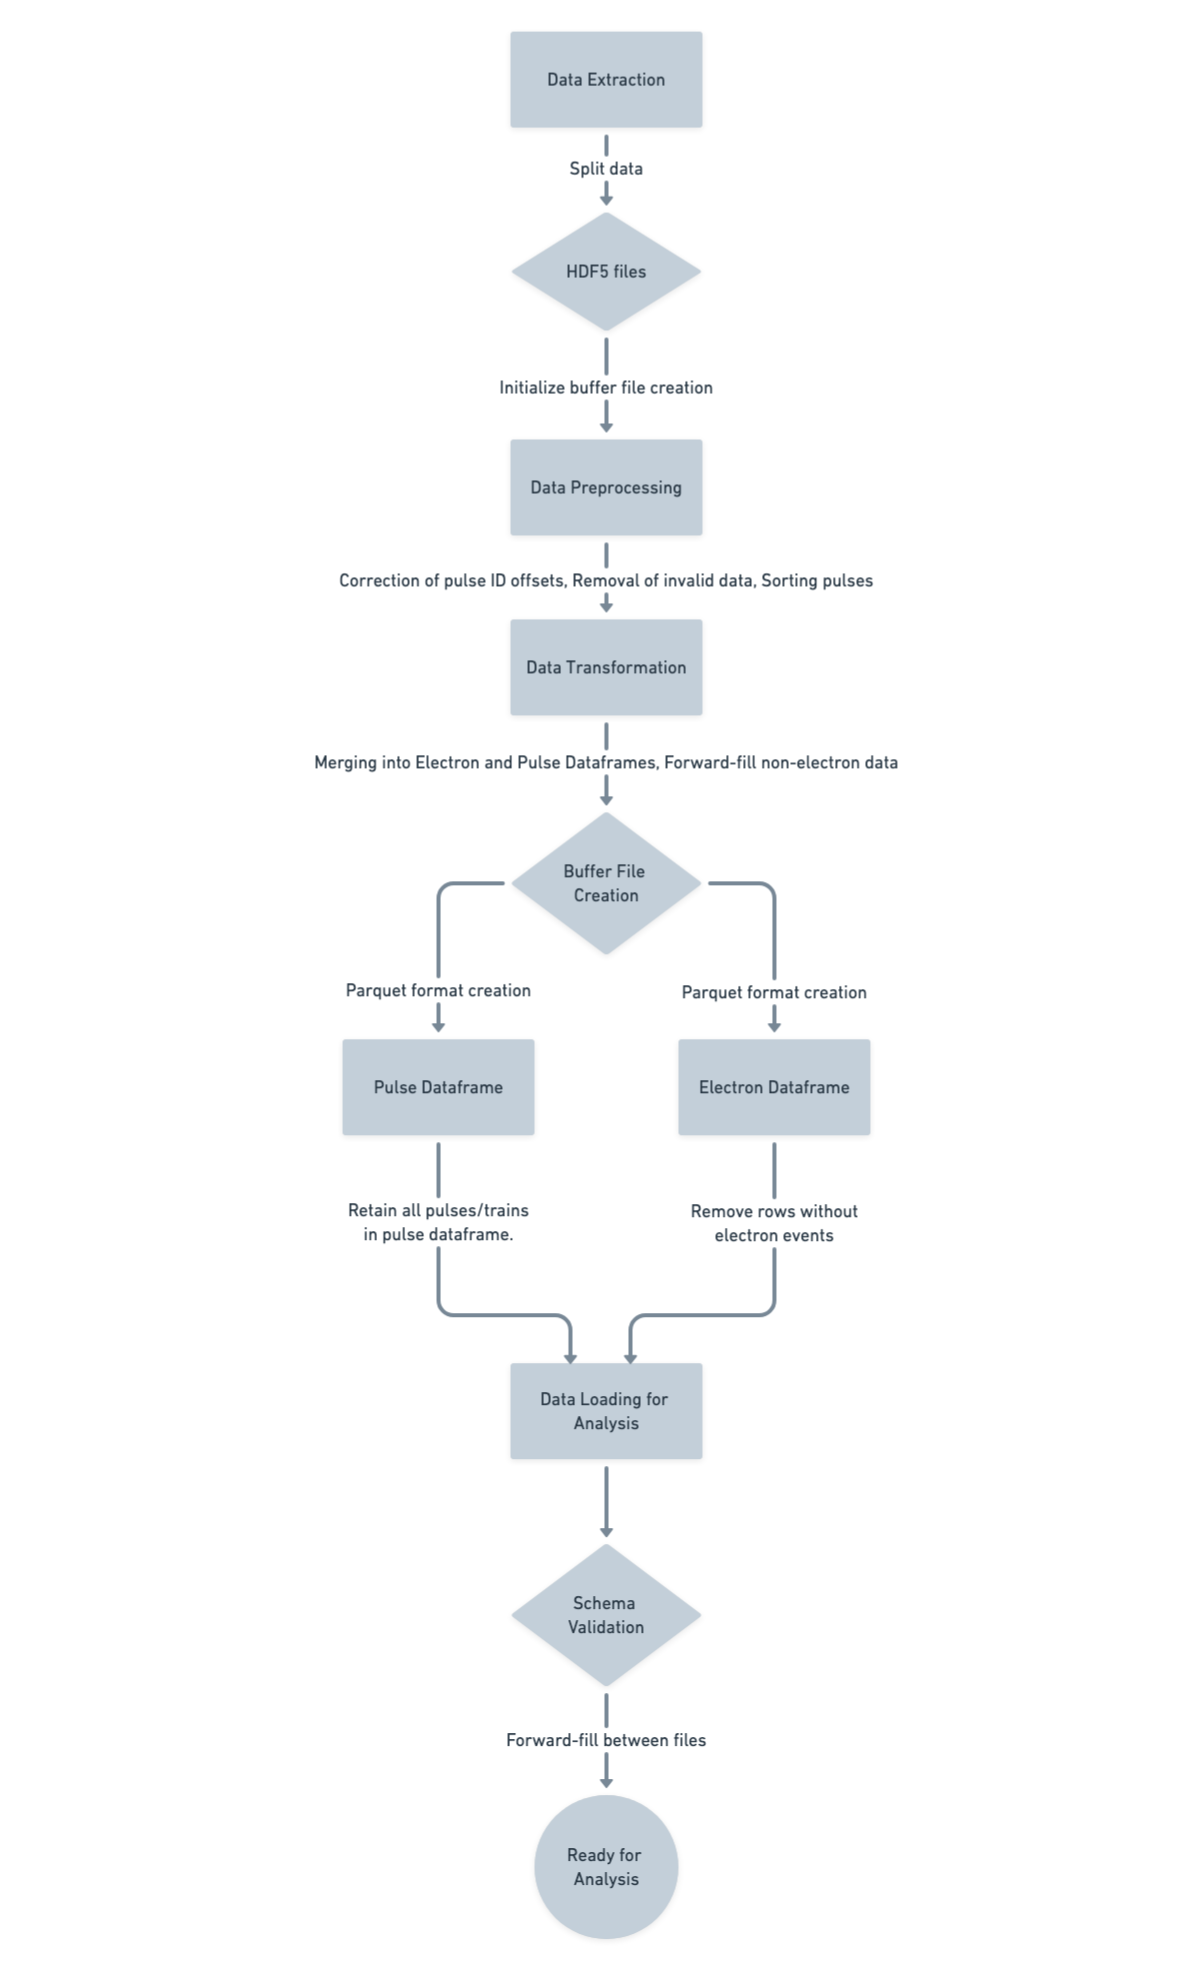
\includegraphics[width=1\linewidth]{images/elt_cropped.png}
    \caption{Complete \gls{ELT} pipeline for the data from \gls{HEXTOF} at \gls{FLASH}}
\end{figure}